% ---------------------------------------------------------------------------- %

\PassOptionsToPackage{dvipsnames}{xcolor}

\documentclass[acmsmall,nonacm,screen]{acmart}

\usepackage[utf8]{inputenc}
\usepackage[T1]{fontenc}

\usepackage{minted}
\usepackage{algorithm}
\usepackage{algpseudocode}
\usepackage{varwidth}
\usepackage{array}
\usepackage{multirow}
\usepackage{stackengine}
\usepackage{blindtext}
\usepackage{enumitem}
\usepackage[portuges]{babel}
\usepackage[toc,page]{appendix}

% ---------------------------------------------------------------------------- %
% configuration

% configure template

\makeatletter
\let\@authorsaddresses\@empty
\makeatother

\makeatletter
\let\ftype@table\ftype@figure
\makeatother

\makeatletter
\setlength{\@fptop}{0pt plus 1fil}
\setlength{\@fpbot}{0pt plus 1fil}
\makeatother

\setlength{\intextsep}{10pt}
\setlength{\textfloatsep}{10pt}

\captionsetup[figure]{name={Figure}}

\setlist{nosep}

% ---------------------------------------------------------------------------- %
% utilities

\makeatletter
\newcommand{\gobblepars}{\@ifnextchar\par{\expandafter\gobblepars\@gobble}{}}
\makeatother

\renewcommand{\paragraph}[1]{%
  \vspace*{.5\baselineskip}%
  \noindent\textbf{#1.} %
  \gobblepars%
  }

\newcommand{\mynote}[3]{%
    {\color{black}%
        \fbox{\bfseries\sffamily\scriptsize#1}%
        {\small$\blacktriangleright$\textsf{\emph{\color{#2}{#3}}}$\blacktriangleleft$}%
    }%
  }

% ---------------------------------------------------------------------------- %
% document

\begin{document}

\title{AA 19/20 -- Relatório Design Patterns 2}
\makeatletter \renewcommand{\shortauthors}{\@title} \makeatother

\begin{abstract}
\large
\vspace*{-.8\baselineskip}
João Marques (A81826), José Pereira (A82880), Ricardo Petronilho (A81744)
\vspace*{.4\baselineskip}
\par \noindent \today
\vspace*{.25\baselineskip}
\end{abstract}

\maketitle

\section{Introdução}
\label{sec:introducao}

\hspace{5mm} O presente relatório relata a investigação sobre \textbf{Design Patterns} no âmbito da Unidade Curricular Arquitecturas Aplicacionais do 4º ano do Mestrado integrado em Engenharia Informática da Universidade do Minho.

\hspace{2mm} O grupo de trabalho decidiu apresentar dois Design Patterns, sendo estes: o \textbf{Memento} e o \textbf{Observer}.

% \hspace{2mm} Primeiro será ilustrado o \textbf{Memento} e de seguida o \textbf{Observer}.
\section{Structural Design Pattern - Decorator}
\label{sec:decorator}

%Não é necessário mais nenhum \hspace
\hspace{3mm} O \textit{Design Pattern} estrutural \textit{Decorator} vem resolver um problema recorrente no desenvolvimento de software, que trata-se da adição de novos comportamentos a objectos, sem necessidade de alterar bastante código, ou aumentar o número de dependências.

Com a finalidade de uma melhor percepção do problema que este design pattern resolve, vai-se seguir um exemplo real referido no website \href{https://refactoring.guru/design-patterns/decorator}{refactoring.guru}. 

Imagine-se um código responsável pela notificação de alguma informação. Deste modo, existirá um cliente e uma classe responsável por essa notificação, sendo neste momento apenas por email. Após o lançamento do produto, verifica-se a necessidade de \textbf{adicionar} novas formas de notificar, tais como: sms, facebook, slack, etc. A primeira solução que poderá ocorrer será utilizar herança, criando subclasses, específicas a cada tipo de notificação, isto é, a classe Email, SMS, Slack, etc..., e estas estenderem a classe responsável pela notificação. No entanto, esta solução contém muitas dependências e um crescimento de subclasses infinito para cada tipo de combinação de notificações, isto é, se se quisesse enviar por exemplo a combinação de SMS + Slack, teria que se criar uma classe específica para tal. Para além destes problemas, muitas linguagens não permitem estender mais do que uma classe, logo utilizar herança será uma má ideia.

Com a finalidade de uma melhor percepção da solução do problema, vai-se usar uma analogia com a realidade. A nível de software a solução para a necessidade de adicionar novas funcionalidades a um objecto, consiste em colocá-lo no "interior"\ de outros, denominados por "\textit{wrappers}".
Em analogia com a realidade, pode-se pensar na boneca \textit{Matriosca}, isto é, a funcionalidade base, consiste na notificação por \textbf{Email}, correspondendo à boneca mais pequena da \textit{Matriosca}. Se for necessário adicionar uma funcionalidade adicional ao \textbf{Email}, por exemplo a notificação por \textbf{SMS}, então vai-se ter uma boneca maior que a do \textbf{Email}, que corresponde ao \textbf{SMS}, e colocar a boneca mais pequena (\textbf{Email}) dentro da boneca do \textbf{SMS}. Ou seja, significa que sempre que se enviar a boneca do \textbf{SMS}, dentro dela vai sempre a boneca do \textbf{Email}, isto é, sempre que se envia o \textbf{SMS}, também se envia o \textbf{Email}.

\begin{figure}[H]
    \centering
    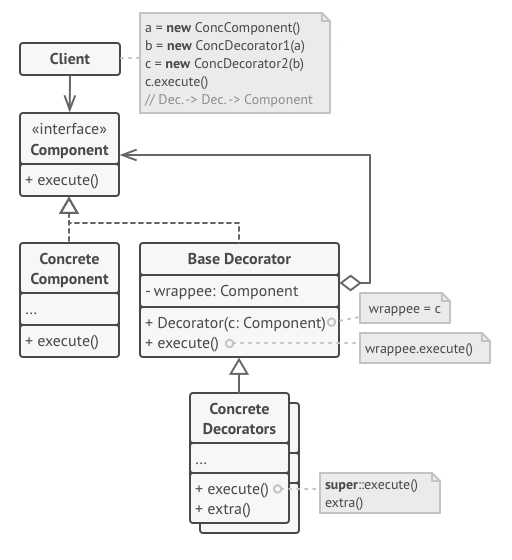
\includegraphics[scale=0.5]{images/decorator.png}
    \caption{Implementação genérica do design pattern Decorator.}
    \label{fig:decorator}
\end{figure}

Após a analogia apresentada anteriormente, explicar-se-á agora em concreto a implementação do design pattern \textit{Decorator}, seguindo a figura \ref{fig:decorator}. A interface \textbf{Component} representa, tanto o \textbf{componente base}, bem como os seus decoradores ("\textbf{decorators}"). Isto é, existem as classes \textbf{ConcreteComponent} e \textbf{BaseDecorator}, que implementam a interface \textbf{Component}, ou seja, uniformizou-se tanto o componente, como os seus decoradores, facilitando desta forma a criação de camadas (análogo ao  \textit{design pattern} \href{https://refactoring.guru/design-patterns/composite}{\textit{Composite}}), como irá ver-se mais adiante. Tal como foi referido, a classe \textbf{ConcreteComponent}, representa o componente base, ou seja, a funcionalidade base (\textbf{execute()}), que no exemplo apresentado consiste na notificação por \textbf{Email}. A classe \textbf{BaseDecorator}, representa todos os \textbf{decorators}, ou seja, faz o "embrulho" (\textit{wrapped)} do componente, através de composição do mesmo (variável \textbf{wrappee}). A forma como se faz o embrulho ao componente é através do envio do mesmo pelo construtor. Importa realçar a importância de se ter definido a interface \textbf{Component}, pois a mesma é que permite a criação de camadas, uma vez que, a variável que está na classe \textbf{BaseDecorator} é do tipo \textbf{Component}, ou seja, tanto pode ser o componente (\textbf{ConcreteComponent}), como um decorador (\textbf{BaseDecorator}). A razão da existência da classe \textbf{BaseDecorator}, consiste, em que todos os \textbf{decorators}, contenham o componente, e a funcionalidade associada a este, uma vez que, o método \textbf{execute} da classe \textbf{BaseDecorator}, chama o \textbf{execute} do componente, tal como se pode verificar nas notas da figura \ref{fig:decorator}. As classes concretas de cada \textbf{Decorator}, vão estender a superclasse \textbf{BaseDecorator}, herdando o método \textbf{execute()} (\textit{override}), e adicionando a este a nova funcionalidade, com o método \textbf{extra()}. Importa realçar ainda, que cada nova funcionalidade extra que se pretenda, basta criar uma nova classe que estenda a \textbf{BaseDecorator}, redefinindo o método \textbf{execute()}, adicionando-lhe a nova funcionalidade.

Por fim, e não menos importante, o cliente, decide como utilizar os \textbf{componentes} e os respectivos \textbf{decoradores}, ou seja, se o cliente apenas necessitar de enviar notificação por email, apenas cria um \textbf{ConcreteComponent}, isto é, uma única camada. Por outro lado, se o cliente, quiser enviar a notificação por email e SMS, terá que criar o \textbf{ConcreteComponent}, de seguida, o decorador do SMS, \textbf{ConcreteDecoratorSMS}, e no construtor deste enviar o componente. De seguida, através da instância do \textbf{ConcreteDecoratorSMS}, chama o método \textbf{execute()}, criando desta forma, duas camadas. Analisando em concreto, o \textit{flow} deste último exemplo, quando no \textbf{ConcreteDecoratorSMS}, chamar o \textbf{execute()}, este irá executar o \textbf{extra()} (funcionalidade adicional), e chamar o \textbf{execute()} do \textbf{BaseDecorator} (utilizando super.execute()), por sua vez, este irá chamar o \textbf{execute()} do \textbf{Component} (funcionalidade base), criando desta forma, duas camadas.

Assim, para uma melhor percepção do \textit{design pattern}, a equipa implementou o mesmo em relação ao problema apresentado das notificações.

\subsection{Notas em relação ao código do Decorator}
\hspace{3mm} O código do \textit{Decorator} encontra-se no anexo \ref{anexo:decorator}. Nos argumentos, bem como no retorno do método \textbf{execute()}, utilizou-se o tipo \textit{Object}, de forma a facilitar a reutilização da interface \textbf{Component}. 

Na classe \textbf{Client} mostra-se três situações de camadas diferentes, sendo respectivamente exemplos de uma, duas e três camadas. No primeiro exemplo, apenas tem-se o componente base, isto é, aquele que envia a notificação por email. De seguida, temos a adição de uma funcionalidade de notificar o cliente por Slack, ou seja, cria-se um decorador, onde se envia o componente base pelo construtor, criando-se duas camadas. Por fim, é feito um exemplo de três camadas, onde em relação ao caso anterior, cria-se mais um decorador, e envia-se, o decorador anterior como argumento, sendo que o decorador anterior, já trás o componente base "dentro" dele. Assim, através do último decorador, chamando o \textbf{execute()}, vai-se notificar em três camadas, isto é, Email, SMS, Slack. 

\section{Behavioral Design Pattern - Mediator}
\label{sec:mediator}

\hspace{3mm} O \textit{Design Pattern} comportamental \textit{Mediator} consiste no \textbf{desacoplamento} dos diversos componentes (objectos) entre si. Desta forma em vez de um objecto comunicar explicitamente com um outro, este fá-lo indirectamente através do \textbf{mediator}.

A implementação genérica do design pattern é a seguinte:

\begin{figure}[H]
    \centering
    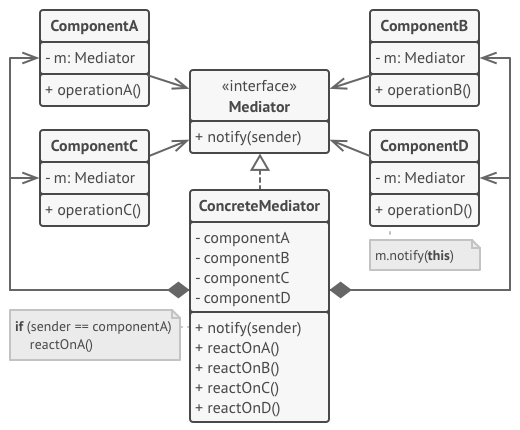
\includegraphics[scale=0.48]{images/mediator_generic_architecture.png}
    \caption{Implementação genérica do design pattern Mediator.}
    \label{fig:mediator}
\end{figure}

Partindo desta arquitectura decidiu-se implementar um exemplo em específico que consiste na gestão de componentes de uma interface gráfica, mais concretamente quando um utilizador clica num botão (Button) é obtido o seu nome, previamente introduzido numa caixa de texto de input (TextInput) e de seguida é apresentada uma mensagem de saudação - "Hello <nome>!" - numa caixa de texto de output (TextBox).

\begin{figure}[H]
    \centering
    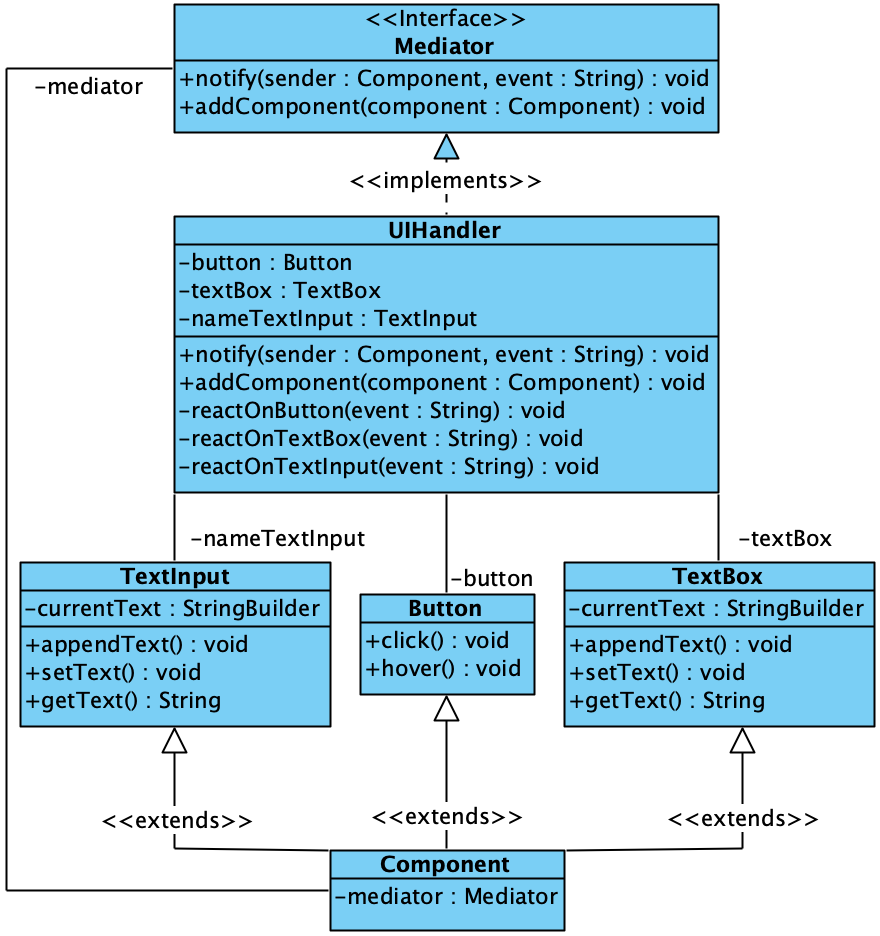
\includegraphics[scale=0.5]{images/class_diagram_mediator.png}
    \caption{Diagrama de classes da implementação.}
    \label{fig:mediator-1}
\end{figure}

A implementação mais fácil, no entanto não a mais correta, seria o botão (Button) conhecer as caixas de texto (TextInput e TextBox), desta forma quando o mesmo fosse clicado simplesmente este acedia à caixa de texto de input (TextInput) para obter o nome e depois à caixa de texto de output (TextBox) para definir a mensagem. \textbf{No entanto, só neste pequeno exemplo, o botão (Button) já tem uma dependência de 1 para 2, sendo que se o botão interagisse com N componentes diferentes essa dependência também aumentava para N}. A manutenção deste código torna-se-ia cada vez mais complicada uma vez que a alteração de um componente ou da forma como esse componente interage com outro poderia exigir a alteração de várias classes.

Uma forma de resolver este problema é a introdução de um objecto mediador (Mediator) que fica responsável pela interacção dos vários componentes entre si. Assim todos os componentes (Button, TextInput e TextBox) \textbf{dependem unicamente do mediador (Mediator), reduzindo assim as dependências de 1 para N para 1 para 1}. Da mesma forma o mediador (Mediator) tem acesso a todos os componentes.

A implementação seria da seguinte maneira, o botão (Button) notifica o mediador (Mediator) que foi clicado (event), de seguida o mediador (Mediator) acede à caixa de texto de input (TextInput) para obter o nome e depois à caixa de texto de output (TextBox) para definir a mensagem. \textbf{Note-se que apesar de se continuar com uma dependência de 1 para N no Mediator, esta dependência é apenas neste objecto}.


\newpage
\section{Anexos}
\label{sec:anexos}

\appendix

\section{Dependency Injection}
\label{anexo:dependency}

\begin{minted}{java}

public interface MessageService {
    void sendMessage(String msg);
}

// ----------------------------------------------------------

public class SMSService implements MessageService {
    @Override
    public void sendMessage(String message) {
        System.out.println("SMS: " + message);
    }
}

// ----------------------------------------------------------

public class EmailService implements MessageService {
    @Override
    public void sendMessage(String message) {
        System.out.println("Email: " + message);
    }
}

// ----------------------------------------------------------

public interface Client {
    void processMessage(String msg);
}

// ----------------------------------------------------------

public class Application implements Client {
    MessageService service;

    public Application(MessageService service) {
        this.service = service;
    }

    @Override
    public void processMessage(String msg) {
        this.service.sendMessage(msg);
    }
}

// ----------------------------------------------------------

public interface MessageServiceInjector {
    public Client getClient();
}

// ----------------------------------------------------------

public class SMSServiceInjector implements MessageServiceInjector {
    @Override
    public Client getClient() {
        return new Application(new SMSService());
    }
}

// ----------------------------------------------------------

public class EmailServiceInjector implements MessageServiceInjector {
    @Override
    public Client getClient() {
        return new Application(new EmailService());
    }
}

// ----------------------------------------------------------

public class Main {
    public static void main(String[] args) {
        String msg = "Hello";
        MessageServiceInjector injector = null;
        Client client = null;

        //Send Email
        injector = new EmailServiceInjector();
        client = injector.getClient();
        client.processMessage(msg);

        //Send SMS
        injector = new SMSServiceInjector();
        client = injector.getClient();
        client.processMessage(msg);
    }
}

// ----------------------------------------------------------

Output:
Email: Hello
SMS: Hello

\end{minted}
\appendix

\end{document}

% ---------------------------------------------------------------------------- %

